\chapter{معماری مدل‌های ارائه شده}
\section{مقدمه}
تاکنون در زبان فارسی، پژوهشگران عمدتاً از مدل‌های مرسوم یادگیری ماشین برای تشخیص اخبار جعلی استفاده کرده‌اند. یکی از اصلی‌ترین دلایل استفاده از این روش‌ها کافی نبودن داده‌های یادگیری برای آموزش مدل‌های به ‌روز و پیچیده است. در این پروژه، پس از جمع‌آوری یک مجموعه داده از اخبار جعلی منتشرشده در پایگاه‌های خبری فارسی، استفاده از مدل‌های عمیق امکان‌پذیر می‌شود. به‌طورکلی پردازش داده متنی در سیستم تشخیص خبر جعلی‌ از دو بخش اصلی بازنمایی متن و دسته‌بندی متن تشکیل شده ‌است که در ادامه توضیح هریک از آن‌ها ارائه می‌گردد.
\section{مدل‌های دسته‌بندی متن}
\subsection{شبکه عصبی پرسپترون ساده}
شبکه عصبی شامل شبکه‌ای از عناصر پردازش ساده (نورون‌ها) است، که می‌تواند رفتار پیچیده کلی تعیین‌شده‌ای از ارتباط بین عناصر پردازش و پارامترهای عنصر را نمایش دهد. این نورون‌ها مجموعه‌ای از ویژگی‌های ورودی را گرفته و باتوجه‌ به ماتریس وزن، تمایل\LTRfootnote{Bias} و تابع فعال‌سازی\LTRfootnote{Activation function} خروجی را به‌دست می‌آورد. \figurename~\ref{fig.slp} نمایی از شبکه عصبی ساده را نمایش می‌دهد.

\begin{figure}[!h]
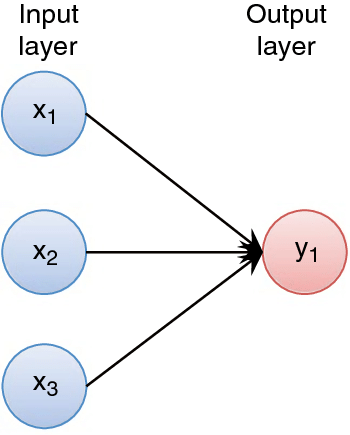
\includegraphics[width=0.25 \textwidth]{slp}
\centering
\caption{نمایی از شبکه عصبی دارای نورون‌های مدل پرسپترون ساده}
\label{fig.slp}
\end{figure}

\begin{table}[!h]
\caption{توابع فعال‌ساز پرکاربرد به‌همراه روابط و نمودار آنها}
\label{table:activationFunctions}
\begin{center}
\begin{tabular}{M{3cm}M{5cm}M{7cm}}
نام & نمودار & تعریف ریاضی \\
\hline
\hline
\lr{Binary step} &
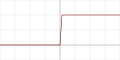
\includegraphics[scale=1]{binary_step} & 
\[f(x) =
\begin{cases}
1, & \verb|x| \geq \verb|0| \\
0, & \verb|x| < \verb|0| \\
\end{cases}
\] \\ \hline

\lr{Sigmoid} &
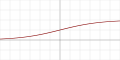
\includegraphics[scale=1]{sigmoid} & 
\[f(x) =
\frac{1}{1 +‌\exp(-x)}
\] \\ \hline

\lr{Tanh} &
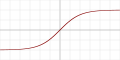
\includegraphics[scale=1]{tanh} & 
\[f(x) =
tanh(x) = \frac{\exp(x) - \exp(-x)}{\exp(x) +‌\exp(-x)}
\] \\ \hline

\lr{Relu} &
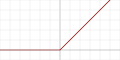
\includegraphics[scale=1]{relu} & 
\[f(x) =
\begin{cases}
x, & \verb|x| \geq \verb|0| \\
0, & \verb|x| < \verb|0| \\
\end{cases}
\] \\ \hline
\end{tabular}
\end{center}
\end{table}


توابع فعال‌ساز با استفاده از ایجاد روابط غیرخطی میان ورودی و خروجی هر نورون سعی می‌کند تا ارتباطات پیچیده‌تری را یاد بگیرد. در \tablename~\ref{table:activationFunctions} چند نمونه از این توابع فعال‌ساز با نمودار مربوط به آنها آورده شده‌است.


%==================================================================
\subsection{شبکه عصبی پیچشی}
این دسته از شبکه‌ها که در ابتدا برای حل مسائل بینایی ماشین ارائه شده بود با به‌کاربستن هسته‌هایی\LTRfootnote{Kernel} با وزن‌های مشترک روی ناحیه‌هایی از ورودی عمل پیچش را انجام می‌دهد. 

 ایده استفاده از وزن‌های‌ مشترک زمانی مطرح شد که تصاویر خاصیت ایستا دارد. این بدان معناست که آماره‌های بخش‌های مختلف یک تصویر و الگوی کلی آنچه که قرار است در تصویر تشخیص داده شود ثابت است و تغییری نمی‌کند. اما استفاده از شبکه‌های پیچشی تنها منحصر به حوزه پردازش تصویر نیست و به‌ مرور وارد سایر حوزه‌ها نظیر پردازش متن نیز شده‌است.
 این نوع شبکه‌ها عمدتاً از لایه‌هایی مانند ادغام\LTRfootnote{Pool} و پیچش\LTRfootnote{Convolution} تشکیل شده‌است. لایه پیچش از فیلترهایی استفاده می‌کند که با
 انجام عملیات پیچش برروی داده ورودی، یک نگاشت ویژگی جدید تولید می‌کند. لایه ادغام نیز معمولاً پس از لایه پیچش،
 برای نمونه‌گیری از نگاشت ویژگی استفاده می‌کند. دو نوع پرکاربرد این نمونه‌گیری، «میانگین مقادیر»\LTRfootnote{Average pooling} و «بیشترین مقدار»\LTRfootnote{Max pooling} است. درنهایت پس‌از به‌دست‌آمدن نگاشت ویژگی نهایی و بردارسازی آن، از یک شبکه عصبی چند لایه استفاده می‌شود تا خروجی
 نهایی باتوجه ‌به ورودی به‌دست آید. از شبکه‌های عصبی پیچشی دو‌ بعدی، عمدتاً برای عکس و از شبکه‌های عصبی پیچشی یک‌بعدی بیشتر برای متن استفاده می‌شود. در \figurename~\ref{fig.alexnet} یک نمونه از شبکه عمیق پیچشی که برای دسته‌بندی عکس استفاده می‌شود نشان داده شده ‌است.

\begin{figure}[!h]
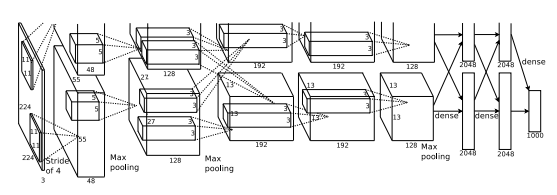
\includegraphics[width=1 \textwidth]{alexnet}
\centering
\caption{نمای کلی مدل پیچشی الکس‌نت \citep{krizhevsky2012imagenet}}
\label{fig.alexnet}
\end{figure}

\vspace{3mm}

\begin{figure}[!h]
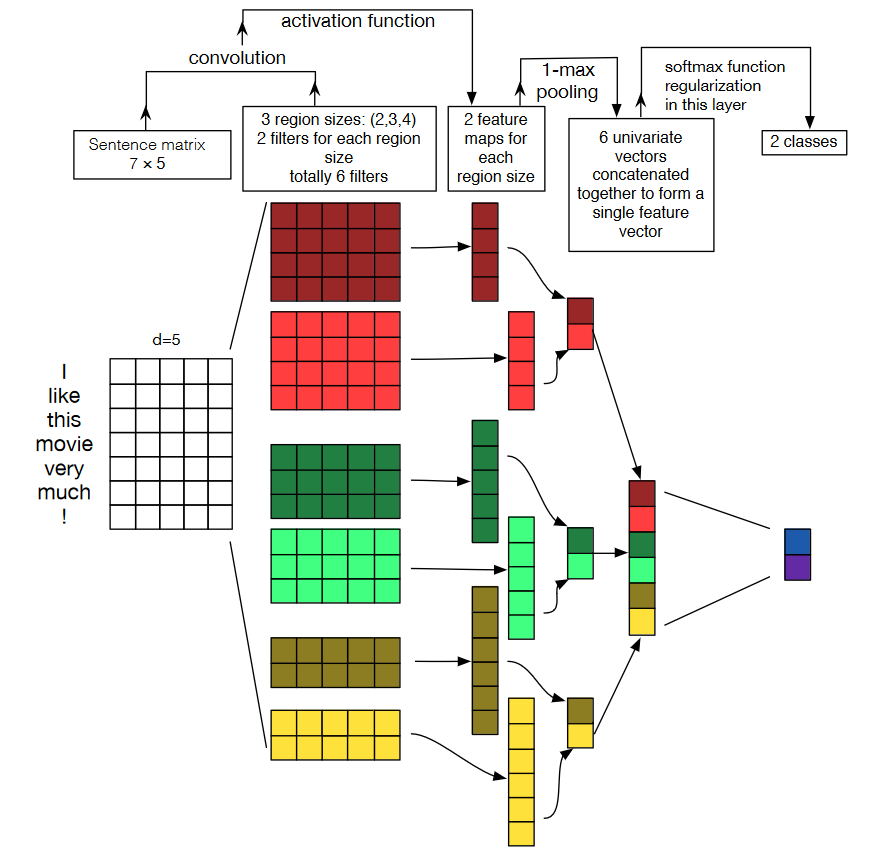
\includegraphics[width=0.85 \textwidth]{cnn}
\centering
\caption{نمای کلی یک شبکه عصبی عمیق پیچشی \citep{le2017convolutional}}
\label{fig.sentimentAnalyzing}
\end{figure}

در ادامه یک مثال کاربردی از شبکه پیچشی در زمینه پردازش متن توضیح داده می‌شود. \figurename~\ref{fig.sentimentAnalyzing} را درنظر بگیرید. یکی از مسائل  پرکاربرد در حوزه پردازش زبان طبیعی، «تحلیل احساسات»\LTRfootnote{Sentiment Analysis} است که در این مثال ما به‌طور خاص  به‌دنبال تشخیص احساس و تمایل در جمله \lr{I like this movie very much.} هستیم. در این مثال کاربردی، داده ورودی به جای یک تصویر، یک ورودی به ابعاد  $n \times d$  است که $n$ طول جمله بر حسب واژه‌ها و $d$ ابعاد تعبیه\LTRfootnote{Embedding} واژه‌ها می‌باشد. سپس در لایه پیچش، روی این ورودی هسته‌هایی با ابعاد مختلف حلقه‌ای زده می‌شود. معمولاً ابعاد این هسته‌ها برای متن ورودی یک بعدی است که این به‌معنای داشتن یک پنجره لغزان روی سطرهای ماتریس می‌باشد. به بیان دیگر، می‌توان این هسته‌ها را بازنمایی سطح بالا از چندتایی‌های واژه‌های ورودی دانست. در لایه بعد، ادغام بیشینه روی خروجی مرحله قبل  انجام شده و خروجی آن‌ها نیز برای دسته‌بندی به لایه تماماً متصل داده می‌شود. در مسئله تحلیل احساس می‌توان فرض کرد که عبارت \lr{like this movie} (که مهم‌ترین عامل نشان‌دهنده احساس است)  در هر جای متن  به‌عنوان احساس مثبت درنظر گرفته‌شده و مکان این عبارت برای تصمیم‌گیری درمورد دسته‌بندی آن اهمیتی ندارد. بنابراین، با حرکت آن پنجره لغزان می‌توان عبارات مثبت را شناخت؛ و درنهایت می‌توان با استفاده از این اطلاعات، مثبت یا منفی بودن احساس کل عبارت را مشخص نمود.

%==================================================================

\section{بازنمایی برداری اخبار با رویکردهای مختلف}
یکی از چالش‌های پردازش زبان طبیعی یافتن یک بازنمایی مناسب برای جملات و یا اجزای کوچکتر آن مانند واژه‌ها است. واژه علاوه بر صورت‌واژه که ازطریق خط تجلی عینی پیدا می‌کند، دارای معنا است که معنای واژه با توجه به بافتی که در آن ظاهر می‌شود تعیین می‌شود. مهم‌ترین عامل تأثیرگذار بر کیفیت یک بازنمایی، شیوه مدل‌سازی معنایی واژه‌ها و یا جملات است. هرچقدر حجم اطلاعات در این بازنمایی بیشتر باشد، بازنمایی دقیق‌تری از واژه یا جمله به‌دست می‌آید. در سال‌های اخیر بازنمایی‌های متفاوتی در حوزه پردازش زبان طبیعی معرفی شده ‌است. در ادامه به توضیح چهار نوع بازنمایی مختلف که به چهار حیطه مختلف اشاره دارد می‌پردازیم. این بازنمایی‌ها عبارت است از: بازنمایی بسامد واژه-معکوس بسامد سند که نوعی بازنمایی پایه مبتنی ‌بر واژه است، بازنمایی تعبیه ایستا ورد2وک که نوعی بازنمایی مبتنی ‌بر معنا براساس هم‌نشینی کلمات است، بازنمایی تخصیص نهان دیریکله که نوعی بازنمایی مبتنی ‌بر موضوع است و مدل‌هایی مانند برت که تحت عنوان بازنمایی‌های مبتنی‌ بر معنای بافت‌محور مطرح می‌شوند.

\subsection{بازنمایی مبتنی ‌بر واژه}
یکی از ساده‌ترین روش‌ها برای بازنمایی اخبار روش مبتنی‌بر واژه است. در این روش با استفاده از شمارش واژه‌های پراهمیت در یک پیکره متنی، یک بازنمایی از آن‌ پیکره ساخته می‌شود. این روش از دو بخش بسامد واژه و معکوس بسامد سند تشکیل شده‌ است. بسامد واژه برابر است با تعداد دفعاتی که یک واژه در یک متن تکرار شده‌ است. البته برای محاسبه این بسامد، فرمول‌های متنوعی وجود دارد. همچنین معکوس بسامد سند به معنای تعداد دفعاتی است که یک اصطلاح در اسناد دیگر به‌کار رفته‌ است که همانند بسامد واژه، روش‌های متنوعی برای محاسبه این معیار وجود دارد که در \tablename~\ref{table.tf} و \ref{table.idf} آورده شده‌ است. $N$ تعداد تمام اسناد، $n_t$ تعداد اسنادی که واژه $t$ در آنها وجود دارد.

\begin{table}[h!]
	\caption{روابط قابل استفاده برای محاسبه بسامد واژه در یک سند}
	\label{table.tf}
	\begin{center}
		\begin{tabular}{|M{5cm}|M{5cm}|}
			\hline
			رویه وزن‌دهی\footnotemark & وزن بسامد واژه \\
			\hline
			\hline
			دودویی\footnotemark & 
			$0, 1$ \\ \hline
			تعداد & 
			$f_{t, d}$ \\ \hline
			بسامد واژه & 
			$ \frac{f_{t,d}}{\sum_{t^{'} \in d} f_{t^{'}, d}}$ \\ \hline
			هنجارسازی لگاریتمی\footnotemark & 
			$\log(1 + f_{t, d})$ \\ \hline
			هنجارسازی دو نیم\footnotemark & 
			$0.5 + ‌0.5\cdot \frac{f_{t, d}}{\max_{t^{'} \in d}{f_{t^{'}, d}}} $ \\ \hline
			هنجارسازی دو کا\footnotemark & 
			$K + (1 - K) \cdot \frac{f_{t, d}}{\max_{t^{'} \in d}{f_{t^{'}, d}}} $ \\ \hline
		\end{tabular}
	\end{center}
\end{table}
\LTRfootnotetext[7]{Weighting scheme}
\LTRfootnotetext[8]{Binary}
\LTRfootnotetext[9]{Log normalization}
\LTRfootnotetext[10]{Double normalization 0.5}
\LTRfootnotetext[11]{Double normalization k}
\begin{table}[h!]
	\caption{روابط قابل استفاده جهت محاسبه معکوس بسامد سند}
	\label{table.idf}
	\begin{center}
		\begin{tabular}{|c|c|}
			\hline
			رویه وزن‌دهی & وزن معکوس بسامد سند \\
			\hline
			\hline
			یگانه & 
			$1$ \\ \hline
			معکوس بسامد سند & 
			$-\log \frac{n_t}{N}$ \\ \hline
			معکوس بسامد سند هموار & 
			$\log(\frac{N}{1 +‌n_t}) + 1$ \\ \hline
			معکوس بسامد سند بیش‌ترین & 
			$\log(\frac{\max_{t^{'} \in d} n_{t^{'}}}{1 +‌n_t})$ \\ \hline
			معکوس بسامد سند احتمالاتی & 
			$\frac{N - n_t}{n_t}$ \\ \hline
		\end{tabular}
	\end{center}
\end{table}

\subsection{بازنمایی مبتنی ‌بر تعبیه ایستا (ورد2وک)}
در روش مبتنی ‌بر واژه،  بر اساس فراوانی و توالی واژه‌های استفاده‌شده در یک پیکره سعی می‌کنیم تا یک بازنمایی مناسب ایجاد کنیم. اما این بازنمایی ارتباط میان اجزای جمله را به‌صورت محدود مدل‌سازی می‌کند. در روش مبتنی‌بر تعبیه ایستا، با استفاده از یک پیکره بزرگ متنی، برای هر واژه یک بازنمایی در اندازه پنجره مشخص ساخته می‌شود. این بازنمایی تا حد قابل قبولی مفاهیم هر واژه را در ساخت بردار در نظر می‌گیرد. خروجی این شیوه بردارسازی به این صورت است که اگر با استفاده از ابزار مصورسازی و کاهش بُعد، یک تصویر از مجموعه واژه‌های یک پیکره را داشته باشیم، اسامی شهر و یا نام ورزش‌های مختلف در نزدیکی هم دیده خواهد شد. علاوه بر این، روابط منطقی نیز میان بردارهای واژه‌ها برقرار است، به‌عنوان مثال، تفاضل بردار واژه‌های «مرد» و «زن» با تفاضل بردار واژه‌های «پادشاه» و «ملکه» برابر است. در بازنمایی ورد2وک، واژه‌ها به فضای برداری نگاشت می‌شود. اگر نیاز به نگاشت اسناد باشد روش داک2وک\LTRfootnote{Doc2vec} و یا میانگین برداری ورد2وک مورد استفاده قرار می‌گیرد. الگوریتم مبتنی‌بر تعبیه ایستا از دو مدل کیسه‌واژه پیوسته\LTRfootnote{Continuous Bag of words} و پرش‌نگاشت\LTRfootnote{Skip-gram}\citep{mikolov2013distributed} استفاده می‌گردد که در ادامه به‌صورت خلاصه آنها را مرور می‌کنیم.

\subsubsection{مدل کیسه‌واژه پیوسته}
برای یادگیری بردار واژه‌ها از همنشینی واژگان در یک پنجره لغزان استفاده می‌شود. در مدل کیسه‌واژه پیوسته، یک واژه به‌عنوان واژه هدف انتخاب شده و به اندازه پنجره لغزان واژه‌های قبل و بعد آن در فرایند یادگیری بردار واژه هدف شرکت می‌کنند. در این مدل هر واژه با استفاده از بازنمایی تک‌روشن به یک شبکه عصبی با یک لایه میانی داده می‌شود و در خروجی انتظار داریم تا احتمال واژه هدف بیشتر از بقیه واژه‌ها باشد. به این صورت مدل  تلاش می‌کند تا واژه هدف را با استفاده از واژه‌های دیگر حدس بزند.

\subsubsection{مدل پرش‌نگاشت}
در مدل کیسه‌واژه پیوسته معنای برخی از واژه‌ها به درستی یادگرفته نمی‌شود؛ چراکه در این میان، تعداد بسیار زیادی از واژه‌های هم‌معنا محو خواهند شد. به همین دلیل، این مدل دقیقا برعکس مدل کیسه‌واژه پیوسته عمل می‌کند تا مشکل معنایی واژه‌های کم تکرار حل شود؛ به این شکل که مدل شبکه عصبی با یک لایه میانی، بردار واژه میانی را دریافت می‌کند و در خروجی، انتظار داریم تا واژه‌هایی که در بافت جایگاهی\LTRfootnote{Local context} اطراف واژه هدف در پنجره لغزان وجود دارد، پیش‌بینی گردد. بنابراین با کاهش هزینه در هر مرحله، مدل تلاش می‌کند تا باتوجه‌به روابط میان واژه‌ها، برداری را برای بازنمایی آنها در لایه میانی یاد بگیرد. ساختار این مدل در \figurename~\ref{fig.skipgram} آورده شده ‌است.

\begin{figure}[h!]
	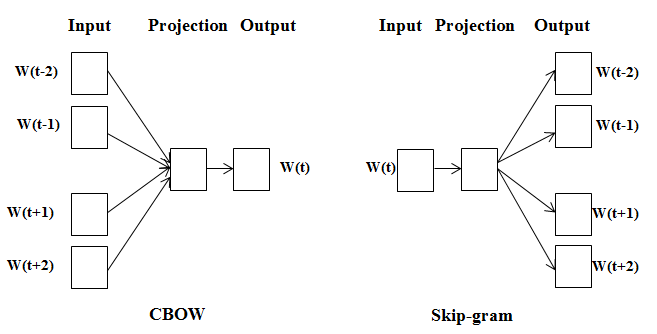
\includegraphics[width=1 \textwidth]{skipgram}
	\centering
	\caption{نمای کلی دو مدل پرش‌نگاشت و کیسه‌واژه پیوسته \citep{suleiman2017deep}}
	\label{fig.skipgram}
\end{figure}


\subsection{بازنمایی مبتنی ‌بر موضوع (تخصیص نهان دیریکله)}
\label{sec:lda}
الگوریتم تخصیص نهان دیریکله\LTRfootnote{Latent Dirichlet allocation (LDA)} یک روش مدل‌سازی بدون‌نظارت برای تعیین موضوعات پیکره متنی است. روش عملکرد مدل‌سازی موضوع به این صورت است که پس از ورود پیکره به این الگوریتم، در نهایت ماتریس سند-موضوع و ماتریس واژه-موضوع ساخته می‌شود. به‌منظور استفاده از این روش برای یافتن یک بازنمایی مناسب برای هر سند می‌توانیم از ماتریس اول استفاده کنیم. هر سطر ماتریس سند-موضوع مرتبط با یک سند است و ستون آن احتمال هر موضوع را نشان می‌دهد. همچنین در ماتریس واژه-موضوع هر ستون یک موضوع است و هر سطر آن نیز امتیاز واژه در آن موضوع است.

\subsection{مدل‌های بازنمائی متن مبتنی بر بافت}
\label{section.pretrained_models}
با معرفی معماری انتفال‌دهنده‌ها  \citep{vaswani2017} طیف وسیعی از مدل‌های زبانی مبتنی بر بافت معرفی شدند. در این بخش به بررسی مدل‌های برت \citep{devlin2018bert} و مدل‌هایی که معماری مشابه برت را دارند مانند برت چند زبانه \LTRfootnote{Multilingual BERT}،
پارس‌برت \LTRfootnote{ParsBERT} \citep{ParsBERT}،
آلبرت‌-فارسی \LTRfootnote{ALBERT-Persian} \citep{ALBERTPersian} و ایکس.ال.ام-روبرتا \LTRfootnote{XLM-RoBERTa} \citep{conneau2019unsupervised} می‌پردازیم.

\subsubsection{برت}
\label{section.bert}
\citet{devlin2018bert} 
یک مدل زبانی جدید با نام برت را معرفی کردند. ایده اصلی این مدل استفاده از انتقال‌دهنده‌های‌\LTRfootnote{Transformer} دوطرفه برای یادگیری معنا و ساختار واژه‌های موجود در متن است. مدل برت به‌صورت دو نسخه «برت پایه»\LTRfootnote{BERT-Base} و «برت بزرگ»\LTRfootnote{BERT-Large} معرفی شده ‌است. برت پایه دارای 12 لایه انتقال‌دهنده و  110 میلیون پارامتر و برت بزرگ دارای  24 لایه و 340 میلیون پارامتر است. انتقال‌دهنده‌ها از «مکانیزم توجه»\LTRfootnote{Attention mechanism} در فرایند یادگیری استفاده می‌کند و سعی می‌کند تا ارتباط مفهومی میان واژه‌های موجود در یک جمله را به‌درستی یاد بگیرد. این مدل برای ایجاد یک بازنمایی مناسب از جملات از ترکیب سه تعبیه استفاده می‌کند که در ادامه توضیحات آنها ارائه می‌شود:
\begin{itemize}
	\item{تعبیه واژه \LTRfootnote{Token Embedding}}: منظور از تعبیه واژه تبدیل هر واژه به فضای برداری یکتا است.
	
	\item{تعبیه جمله \LTRfootnote{Sequence Embedding}}: هر داده ورودی مدل برت از دو جمله "آ`` و "ب`` تشکیل شده‌است که در یکی از مراحل یادگیری، این مدل برای پیش‌بینی جمله بعدی کاربرد دارد. به همین منظور، این مدل یک تعبیه برای مشخص‌کردن جمله‌ای که واژه مورد نظر در آن قرار دارد، ایجاد می‌کند.
	\item{تعبیه موقعیت انتقال‌دهنده‌ها \LTRfootnote{Transformer Positional Embedding}}: تعبیه موقعیت انتقال‌دهنده‌ها یک تعبیه از موقعیت هر واژه در جمله است که باعث می‌شود بردار حضور هر واژه در جایگاه‌های مختلف در یک جمله متفاوت باشد.
\end{itemize}

درنهایت با ترکیب این سه بخش، یک بردار ورودی برای مدل برت ساخته می‌شود که پس از مراحل یادگیری گفته‌شده در بخش قبل، برای هر جمله یک بازنمایی مناسب ارائه می‌یابد. شکل \ref{fig.bert_embedding} ساختار این روش را نمایش می‌دهد.

\begin{figure}[!h]
	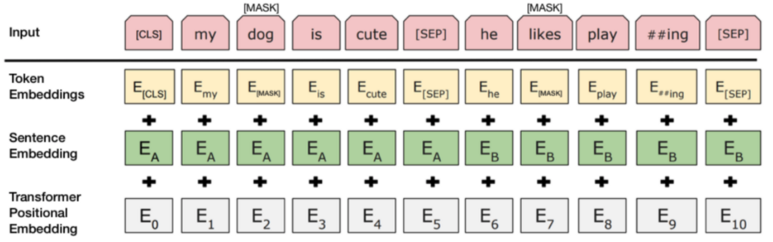
\includegraphics[width=1 \textwidth]{bert_embedding}
	\centering
	\caption{نحوه ترکیب تعبیه‌های سه‌گانه در مدل زبانی برت \citep{devlin2018bert}}
	\label{fig.bert_embedding}
\end{figure}
%%%%%%%%%
 فرایند یادگیری مدل‌های زبانی عموماً به این صورت است که تلاش می‌کند تا واژه بعدی یک دنباله را حدس بزند و بر این اساس، ارتباط میان واژه‌ها را تشخیص دهند. اما در مدل زبانی برت که به‌صورت دوطرفه (چپ‌به‌راست و راست‌به‌چپ) متن را بررسی می‌کند نمی‌توان فقط از این روش استفاده کرد. 
همچنین برای آموزش مدل برت دو مرحله اصلی برروی پیکره‌های متنی ویکی‌پدیا و کتاب‌ها اعمال شده‌است که در ادامه با آن‌ها آشنا می‌شویم. 
 در \figurename~\ref{fig.BERT} نحوه آموزش در مدل برت نمایش داده شده‌است.

\begin{figure}[!h]
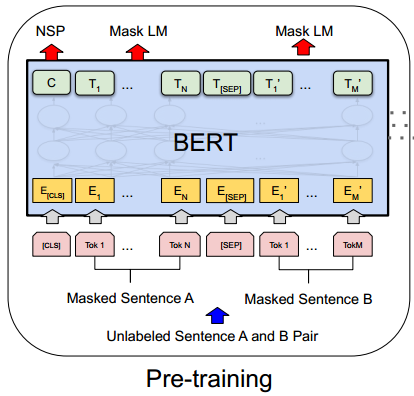
\includegraphics[width=0.6 \textwidth]{bert}
\centering
\caption{ نحوه عملکرد یادگیری مدل برت \citep{devlin2018bert}}
\label{fig.BERT}
\end{figure}

\begin{itemize}
\item \textbf{پوشش واژه‌ها} \\
قبل از استفاده از داده‌ها در شروع فرایند یادگیری، 15 درصد از واژه‌های داخل متن به‌صورت تصادفی انتخاب می‌شود. 
 از این حجم واژه‌ها 80‌ درصد واژه‌ها با عبارت \verb|[MASK]| جایگزین شده و 10 درصد با یک واژه تصادفی جایگزین می‌شود و 10
 درصد دیگر بدون تغییر باقی می‌ماند. در ادامه، مدل سعی می‌کند تا با استفاده از اطلاعات زمینه‌ای، این واژه‌ها را حدس بزند.
 این کار با اضافه‌کردن یک لایه پس از لایه کدگذار مدل برت انجام می‌شود تا با استفاده از آن، احتمال وجود هریک از واژه‌ها
 مشخص شود و با داشتن واژه اصلی، خطای مدل حساب شده و تمامی وزن‌ها به‌روزرسانی می‌شود.

\item \textbf{پیش‌بینی جمله بعدی} \\
در این حالت، مدل برت یک جفت دنباله مانند "آ`` و "ب`` را دریافت می‌کند. در ابتدا و انتها جملات عبارات \verb|[CLS]| و \verb|[SEP]| قرار
 می‌گیرد. پس از اضافه‌کردن نوع جمله ("آ`` یا "ب``) به ویژگی‌های نهفته هر جمله، تمامی ورودی‌ها وارد انتقال‌دهنده‌ها شده و درنهایت با استفاده از یک لایه، مقدار احتمال ظهور دنباله "ب`` به‌عنوان جمله بعدی دنباله "آ`` مشخص می‌شود. با این روش مدل برت تلاش می‌کند تا مفاهیم زمینه‌ای را به‌طور کامل میان واژه‌ها و عبارات یاد بگیرد.
\end{itemize}

درنهایت پس از آماده‌شدن مدل زبانی، می‌توانیم از آن در مسائل مختلف مانند دسته‌بندی متن، پرسش و پاسخ\LTRfootnote{Question Answering (QA)} و تشخیص
 موجودیت‌های نامدار\LTRfootnote{Name Entity Recognition (NER)} استفاده کنیم.


\subsubsection{برت چند زبانه}
	مدل زبانی برت چند زبانه \citep{devlin2018bert} با استفاده از داده‌هایی از ۱۰۴ زبان مختلف شامل زبان فارسی آموزش داده شده‌است. مدل زبانی برت دارای دو نوع پایه و بزرگ است که ما در این پروژه از مدل برت پایه، شامل ۱۲ لایه انتقال‌دهنده و ۱۱۰ میلیون پارامتر استفاده کرده‌ایم. این مدل با استفاده از پیکره متنی ویکی‌پدیا\LTRfootnote{Wikipedia} که به زبان‌های مختلف موجود است، آموزش داده شده ‌است. 
	
\subsubsection{پارس‌برت}
	\cite{ParsBERT}
	مدل زبانی پارس‌برت که مبتنی بر معماری مدل برت است، انحصاراً برای زبان فارسی آموزش دادند. این مدل عملکرد بهتری نسبت‌به مدل‌های چند زبانی مانند برت داشته ‌است. همچنین به‌دلیل آنکه این مدل تنها برای زبان فارسی ارائه شده‌ است، سبک‌تر از مدل زبانی برت چندزبانه است. به‌منظور آموزش مدل‌زبانی پارس‌برت از منابع متنی موجود در وب‌سایت‌های ویکی‌پدیا، بیگ‌بنگ، چطور، الی‌گشت، دیجی‌کالا، تد‌تاک، کتاب‌ها و پیکره میراث استفاده شده‌است. همچنین برای ارزیابی مدل‌ ارائه‌شده در پارس‌برت از تحلیل احساسات، تشخیص موجودیت‌های نامدار و دسته‌بندی متن استفاده شده ‌است.
	
\subsubsection{آلبرت-فارسی}
	مدل‌ زبانی آلبرت یک نسخه سبک‌تر از برت است که معماری کاملاً مشابه‌ای با آن دارد که در پیاده‌سازی آن تغییر اندکی نسبت ‌به مدل برت وجود دارد \citep{ALBERTPersian}. آلبرت-فارسی، مانند مدل‌زبانی پارس‌برت بر روی  پیکره‌های متنی فارسی آموزش داده شده‌ است. علیرغم اینکه منابع این پیکره‌های فارسی مشابه مدل‌زبانی پارس‌برت است، به ‌مراتب حجم  کمتری نسبت ‌به پارس‌برت دارد.
	
\subsubsection{ایکس.ال.ام-روبرتا}
	با توجه به موفقیت‌های چشمگیر مدل‌های ازپیش آموزش‌دیده، \cite{conneau2019unsupervised} یک مدل‌ بین‌زبانی ارائه کردند که توانست دقت بهتری را در مقایسه با مدل‌های زبانی رایج مانند برت ثبت کند. این مدل که بر روی دادگان ۱۰۰ زبان مختلف ازجمله فارسی آموزش داده شده‌ است  با استفاده از ۳ روش آموزش داده می‌شود: (۱) پیش‌بینی کلمه بعدی، (۲) پیش‌بینی کلمه پوشیده شده و (۳) مدل زبانی مبتنی بر ترجمه.
%==================================================================

\section{معماری‌های پیشنهادی برای تشخیص اخبار جعلی}
به طور کلی، مدل‌های بازنمائی متن مبتنی بر بافت خروجی‌های متفاوتی را می‌توانند ایجاد کنند. مدل‌هایی با ساختار مشابه برت مانند پارس‌برت، آلبرت-فارسی و برت چند زبانه ۲ نوع بازنمائی برای متن ورودی ایجاد می‌کنند:
\begin{itemize}
\item بازنمایی تجمعی\LTRfootnote{Pooled} به ازای هر دنباله از واژه‌های ورودی، یک بازنمایی کلی برای کل دنباله ارائه می‌کند.
این بازنمائی تنها توسط مدل‌های مبتنی بر ساختار برت ایجاد می‌شود.
\item بازنمایی دنباله‌ای\LTRfootnote{Sequence} که در آن برای هر واژه یک بردار بازنمایی مبتنی‌بر بافت ارائه
 می‌گردد. برخلاف بازنمائی تجمعی، بازنمائی دنباله‌ای را تمامی مدل‌های بازنمائی متن مبتنی بر بافت تولید می‌کنند.
\end{itemize}

در این پروژه، دو معماری مختلف مورد استفاده قرار گرفته‌است که در هر یک از این معماری‌ها، یکی از دو حالت فوق به‌کار رفته‌است. در روش اول با استفاده از یک مدل پرسپترون ساده به دسته‌بندی اخبار بازنمائی شده توسط بردار‌های تجمعی می‌پردازیم و در روش دوم با استفاده از بازنمائی دنباله‌ای و یک شبکه‌‌عصبی پیچشی به استخراج ویژگی‌های سطح بالاتر از هم‌نشینی واژگان یک خبر می‌پردازیم و درنهایت با استفاده از یک لایه چگال، اخبار دسته‌بندی می‌شوند.


%==================================================================

\subsection{مدل زبانی مبتنی بر بافت + پرسپترون ساده}
برای استفاده از مدل‌‌های مبتنی بر بافت در مسئله دسته‌بندی کافی است تا از بردار خروجی متناظر با توکن \verb|[CLS]| به‌عنوان بردار نماینده آن دنباله استفاده کنیم. دلیل استفاده از این بردار این است که شامل تمامی بردارهای توکن‌های موجود در متن است، درحالی‌که بردارهای متناظر با توکن‌های دیگر تنها نماینده آن توکن در عبارت ورودی است. بنابراین کافی است تا بردار نماینده دنباله متنی ورودی را وارد یک لایه تکی پرسپترون کنیم که می‌تواند عمل تشخیص برچسب دنباله ورودی را برای ما انجام دهد. این ساختار با استفاده از مدل زبانی برت در \figurename~\ref{fig.bertSLP} ترسیم شده‌است.

به عبارت دیگر، با استفاده از بازنمایی به‌دست‌آمده از مدل برت برای یک جمله و داشتن برچسب آن سعی می‌کنیم تا با استفاده از  دادگان موجود، یک مدل کامل برای تشخیص اخبار جعلی بسازیم. برای این هدف کافی است تا وزن‌های ورودی به لایه پرسپترون  ساده آموزش داده شود به صورتی که بتواند اخبار را به درستی دسته‌بندی کند. 

\begin{figure}[!h]
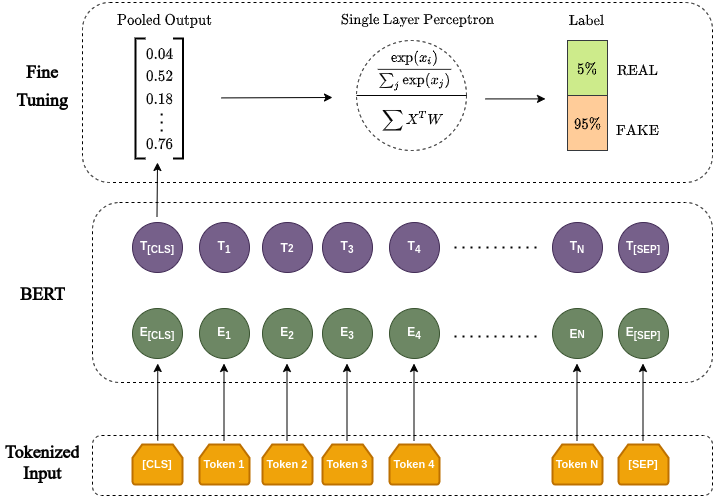
\includegraphics[width=0.75 \textwidth]{bert_slp}
\centering
\caption{نحوه استفاده از یک لایه پرسپترون ساده درکنار مدل برت}
\label{fig.bertSLP}
\end{figure}
\noindent

به‌منظور جلوگیری از «بیش‌برازش»\LTRfootnote{Overfitting} مدل، از روش «حذف تصادفی نورون‌ها»\LTRfootnote{Dropout} استفاده می‌کنیم تا مدل نهایی تا حد ممکن ساده باشد و به‌درستی ویژگی‌های مهم را یاد بگیرد. در انتهایی‌ترین بخش مدل هم یک لایه نورون به تعداد دسته‌های دادگان ورودی وجود دارد که تابع فعال‌ساز آنها «بیشینه نرم»\LTRfootnote{Softmax} است چراکه نیاز داریم تا احتمال تعلق‌داشتن خبر به هر دسته را بدانیم و بیشترین آن را به‌عنوان برچسب پیش‌بینی ‌شده اعلام نماییم.

تابع «خطا آنتروپی متقاطع طبقه‌ای»\LTRfootnote{ Categorical Cross-entropy} نیز برای محاسبه میزان خطای پیش‌بینی مدل دسته‌بند خبر جعلی استفاده شده ‌است که رابطه ریاضی آن در ادامه آورده شده است.

\begin{equation}
Loss = - \sum_{c=1}^{M}y_{o,c} . log(p_{o,c})
\end{equation}
در این رابطه، $M$ تعداد دسته‌ها و $y_o$ بردار تک‌روشن از برچسب خبر $o$ است و $p_o$ نیز بردار احتمال پیش‌بینی‌شده توسط مدل است که نشان‌دهنده احتمال تعلق به هر دسته است.

%==================================================================

\begin{figure}[!t]
	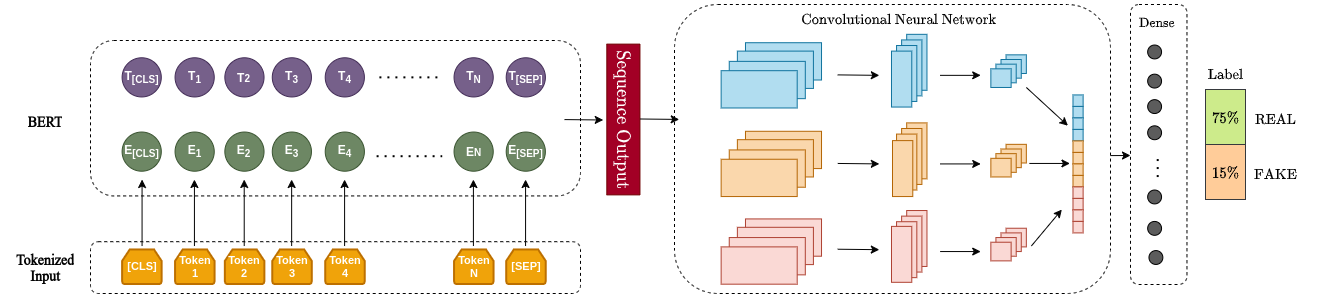
\includegraphics[width=1 \textwidth]{bert_cnn}
	\centering
	\caption{نحوه ارتباط لایه پیچشی با بردارهای خروجی مدل برت}
	\label{fig.bertCNN}
\end{figure}

\subsection{مدل زبانی مبتنی بر بافت + پیچشی}
\label{sec:bert_cnn}
با استفاده از خروجی دنباله‌ای یک مدل‌ بازنمائی مبتنی بر بافت و اتصال آن به یک شبکه عصبی پیچشی، عملیات نگاشت ویژگی انجام داده می‌شود. پس‌از عملیات یادگیری، این مدل سعی می‌کند تا با تبدیل بازنمایی تولیدشده به یک بازنمایی دیگر، عملیات پیش‌بینی کذب‌بودن یا اصیل‌بودن یک خبر را انجام دهد. در این مدل، به‌جای بردار خروجی تجمعی، از بردار خروجی دنباله‌ای که شامل دنباله‌ای از بردارهای تک‌تک واژه‌های داخل خبر است استفاده می‌گردد؛ چراکه با استفاده از لایه‌های پیچشیِ پس‌از آن می‌توان همنشینی‌هایی از واژه‌ها که نشان‌دهنده اخبار جعلی است را شناسایی کرد. برای این منظور، از سه لایه پیچشی موازی شامل ۳۰ فیلتر با اندازه‌های ۳، ۴ و ۵ استفاده می‌کنیم. همچنین تابع فعال‌ساز این لایه، تابع «یک‌سوساز خطی»\LTRfootnote{ReLU} است. پس از این لایه، یک لایه ادغامِ بیشترین مقدار قرار دارد تا با استفاده از عملیات «نمونه‌کاهی»\LTRfootnote{Downsampling}، ویژگی‌های مناسب را استخراج کند. درنهایت، با استفاده از یک «لایه مسطح‌شده»\LTRfootnote{Flatten layer}، ماتریس مرحله قبل به یک بردار یک بعدی تبدیل می‌شود تا با استفاده از یک لایه چگال\LTRfootnote{Dense} با استفاده از تابع فعال‌ساز «بیشینه نرم»، احتمال هر دسته مشخص شود. \figurename~\ref{fig.bertCNN} نحوه اتصالات و به‌دست‌آوردن ویژگی‌های سطح بالاتر با استفاده از مدل زبانی برت را نشان می‌دهد.